\section{Conclusion}
	\begin{itemize}
			\item \todo{We need a coordination at the language level, explicit by using a dedicated language and that enables the verification and validation of the coordinated system}
			
			\item \todo{The knowledge about system integration is currently either implicitly held by the integrator or encoded within a framework. To capture explicitly this knowledge and thus leverage integrator know-how, we propose a dedicated language to capture coordination patterns between languages, thus reifying the coordination specification at the language level.}
			
		\item In this chapter, we have presented a background of the pivotal concepts used in the
		following chapters. We have introduced the architecture concept visualized in the system
		domain. Afterwards, we have presented the multi-view modeling vocabulary specified
		in the IEEE-42010 standard and its relationship with MDE. We have noted that
		a viewPoint is a DSML in the MDE context. We have identified the connection between
		the multi-view approaches and model composition. We have determined that
		the model composition work could be used in the multi-view approach to characterize
		the correspondence rules and their interpretations. We have presented some works that
		implement these approaches (multi-view and model composition) and we have identified
		the correspondences and their interpretations according to Clavreul’s work.
		We have continued with the behavioral definition in the multi-view approach. The
		importance to separate semantics and syntax in the definition of a viewPoint has been
		highlighted. MoCs are adopted as the modeling approach to specify the semantic domain
		in a viewPoint. We stressed the importance of behavioral correspondences in addition
		to purely structural correspondences in the multi-view modeling. Such behavioral correspondences
		are bound to the heterogeneous behavior associated with MoC interactions.
		We have presented two approaches (hierarchy and automaton based) frequently used to
		specify the interactions between MoCs.
		In the next chapter, we use the concepts from this chapter to define a multi-view framework
		to model systems
	\end{itemize}


         	\begin{figure}
         		\begin{center}
         			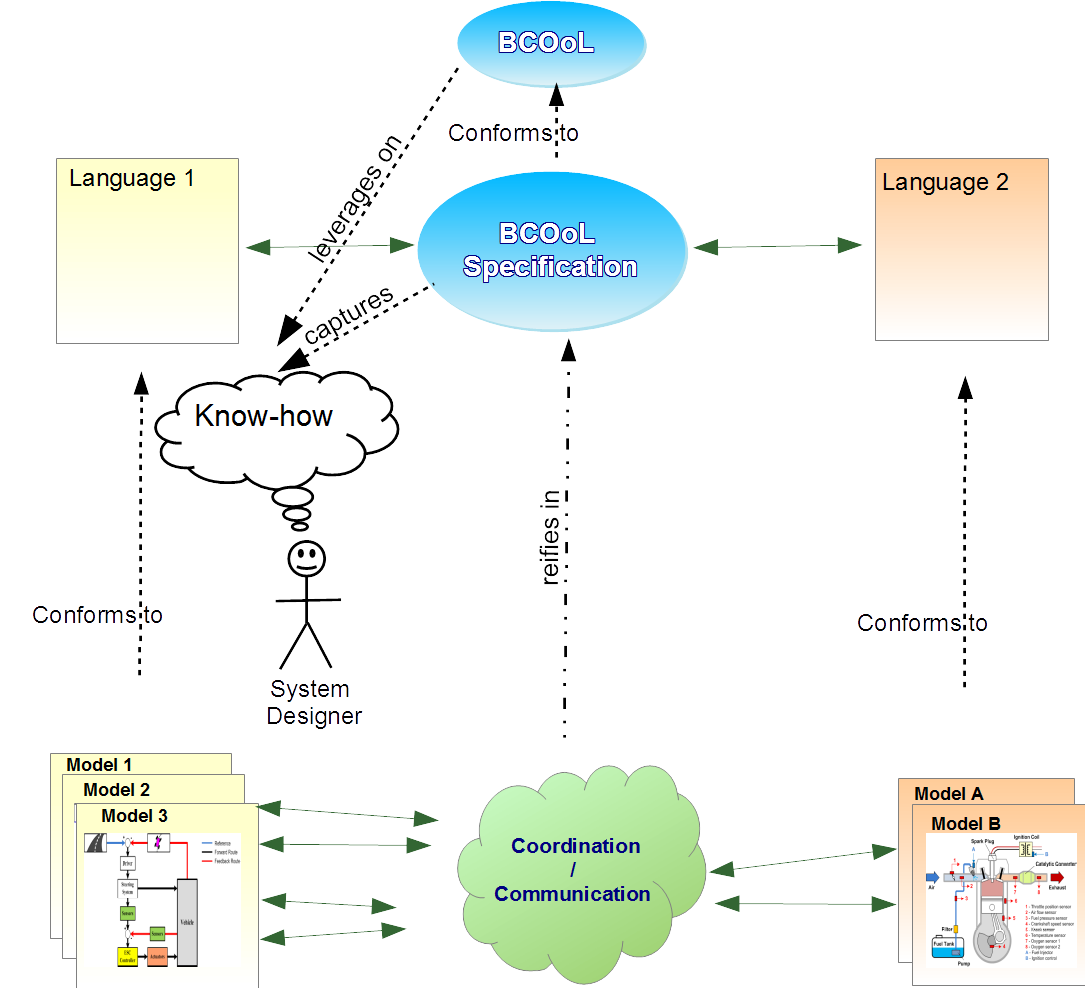
\includegraphics[width=0.7\textwidth]{background/figs/bcoolapp.png}
         			\caption{Overview of Our Approach}
         			\label{fig:diNatale}
         		\end{center}
         	\end{figure}	

\begin{table}[h]
	\centering
	\caption{Overview of state of art approaches}
	\label{my-label}
	\begin{tabular}{cccccc}
		\multicolumn{1}{l}{\multirow{2}{*}{Approach}} & \multicolumn{1}{l}{\multirow{2}{*}{Syntactic Composition}} & \multicolumn{2}{c}{Semantics Composition} & \multirow{2}{*}{Specification} & \multirow{2}{*}{Application} \\
		\multicolumn{1}{l}{}                          & \multicolumn{1}{l}{}                                       & Composition         & Coordination        &                                &                              \\
		Epsilon                                       & Yes                                                        &                     &                     & Lenguage Level                 & Model Level                  \\
		Ptolemy\cite{ptoleframebib}                                      & No                                                         &                     & X                   & Language Level                 & Model Level                  \\
		Rapide                                        & No                                                         &                     & X                   & Model Level                    & Model Level                  \\
		Esper                                         & No                                                         &                     & X                   & Model Level                    & Model Level                  \\
		MASCOT                                        & No                                                         &                     & X                   & Language Level                 & Model Level                  \\
		\cite{compostatechartsbib}                  & No                                                         & X                   &                     & Language Level                 & Model Level                      
	\end{tabular}
			\todo{To use one page and put all studied approaches}
\end{table}